\documentclass[12pt, a4paper]{article}
\usepackage[top=1.0in, bottom=1.0in, left=0.8in, right=0.8in]{geometry}

\setlength{\parskip}{\baselineskip}%
\setlength{\parindent}{0pt}%
\usepackage{bookmark}
\usepackage[]{graphicx}
\usepackage{enumitem}
\usepackage{amsmath}
\usepackage{relsize}
\usepackage{cprotect}
\usepackage{amsmath, amsfonts}
\usepackage{siunitx}
\usepackage{mathrsfs}
\usepackage{framed}
\usepackage{enumitem}
\usepackage{tikz}
\usepackage{circuitikz}
\usepackage{float}
\usepackage[english]{babel}
\usepackage{blindtext}

\newlist{notes}{enumerate}{1}
\setlist[notes]{label=\textbf{Note:} ,leftmargin=*}

\newlist{hints}{enumerate}{1}
\setlist[hints]{label=\textbf{Hint:} ,leftmargin=*}

\usepackage{xcolor}
\usepackage{color}
\definecolor{com1}{RGB}{125,125,125}
\definecolor{comment}{RGB}{140,115,115}
\definecolor{numbering}{rgb}{0.2,0.2,0.2}
\definecolor{key}{RGB}{0,0,180}
\definecolor{in}{RGB}{0,100,0}
\definecolor{out}{RGB}{100,30,30}
\definecolor{bg}{RGB}{245,245,245}
\definecolor{bgLight}{RGB}{250,250,250}
\definecolor{string}{RGB}{0,150,0}

\usepackage{hyperref}
\hypersetup{
    colorlinks=true,
    linkcolor=blue,
    filecolor=magenta,      
    urlcolor=blue,
}
\urlstyle{same}

\usepackage{listings}

\lstdefinestyle{py_code}{ %
    backgroundcolor=\color{bg},      % choose the background
    basicstyle=\ttfamily\small,		      % fonts
    breakatwhitespace=false,         % automatic breaks at whitespace ?
    breaklines=true,                 % sets automatic line breaking
    captionpos=b,                    % caption-position - bottom
    commentstyle=\itshape\color{comment},    % comment style
    extendedchars=true,              % use non-ASCII
    frame=single,	                   % single frame around the code
    keepspaces=true,                 % keeps spaces in text
    keywordstyle=\bfseries\color{key},% keyword style
    language=Python,                 	  % the language of the code
    morekeywords={Null},       % add more keywords to the set
    numbers=left,                    % line_numbers (none, left, right)
    numbersep=10pt,                  % line_no - code dist
    numberstyle=\footnotesize\color{numbering}, % line_no style
    rulecolor=\color{black},         % frame_color [!always set]
    showspaces=false,                % show spaces everywhere
    showstringspaces=false,          % 
    showtabs=false,                  % 
    stepnumber=1,                    % step b/w two line-no
    stringstyle=\color{string},     % string literal style
    tabsize=2,	                       % sets default tabsize to 2 spaces
    title=\lstname,                  % show the filename
    escapeinside={(*}{*)},			  % escape from style inside (* *)
    xleftmargin=\parindent,
    belowskip=-1.3 \baselineskip,
    aboveskip=1.0 \baselineskip,
    columns=fullflexible,
    xleftmargin=0.15in,
}
\lstnewenvironment{py_code}
{\lstset{style=py_code}}
{}

\lstdefinestyle{psudo}{ %
    backgroundcolor=\color{bgLight},   % choose the background
    basicstyle=\ttfamily\small,		      % fonts
    breakatwhitespace=false,         % automatic breaks at whitespace ?
    breaklines=true,                 % sets automatic line breaking
    captionpos=b,                    % caption-position - bottom
    commentstyle=\itshape\color{com1},          % comment style
    extendedchars=true,              % use non-ASCII
    keepspaces=true,                 % keeps spaces in text
    language=C,                 	  % the language of the code
    morekeywords={type,NULL, True, False},       % add more keywords to the set
    showspaces=false,                % show spaces everywhere
    showstringspaces=false,          % 
    showtabs=false,                  % 
    tabsize=2,	                       % sets default tabsize to 2 spaces
    title=\lstname,                  % show the filename
    escapeinside={(*}{*)},			  % escape from style inside (* *)
    belowskip=-1.8 \baselineskip,
    aboveskip=0.9 \baselineskip,
    columns=fullflexible,
    xleftmargin=0.2in,
    frame=tb,
    framexleftmargin=16pt,
    framextopmargin=6pt,
    framexbottommargin=6pt, 
    framerule=0pt,
}

\lstnewenvironment{psudo}
{\lstset{style=psudo}}
{}

\graphicspath{ ./ }

\title{\textbf{EE2703 : Applied Programming Lab \\ Assignment 6 \\ The Laplace Transform}} 
\author{Chagari Koushal Kumar Reddy \\ EE20B023} % Author name

\date{\today} % Date for the report

\begin{document}		

\maketitle % Insert the title, author and date
\clearpage

\tableofcontents
\clearpage

\section{Aim}
The aim of this assignment is to :
\vspace{-0.3cm}
\begin{enumerate}
    \item Learn about the scipy.signal library and polynomial functions of the numpy
    library
    \item Use those tools to solve various Linear constant coefficient Differential Equations using Laplace Transform techniques
\end{enumerate}
\section{Theory: Laplace Transform}
Laplace transform is a powerful technique used in electrical engineering to solve complex
mathematical differential equations. This technique helps us to solve various
real-life problems such as:
\vspace{-0.3cm}
\begin{enumerate}
    \item Steady state response of an electrical circuit
    \item Steady state response of a mechanical spring block system
    \item Analyzing the behaviour of electrical filters
\end{enumerate}
The formula for unilateral laplace transform of a continous time function $x(t)$ is given by:
\begin{equation*}
    X(s) = \int_{0}^{\infty} x(t)dt
\end{equation*}
where s is the complex frequency. One major use of Laplace transform is that if $x(t)$ gives $X(s)$, then $\frac{dx(t)}{dt}$ gives $sX(s)$ provided that initial conditions are zero.
Also Laplace transform is a linear transform. These 2 properties will help us solve differential equations easily in the laplace domain as they will be converted to algebraic equations.
\section{Assignment Objectives}
\vspace*{-0.5cm}
\subsection{Response of a spring-mass system}
The differential equation of a spring-mass system is given as:
\begin{equation*}
    \ddot x + \omega _{o}^{2}x = f(t)
\end{equation*}
with $f(t) = cos(\omega _{d}t)\exp ^{-at}u(t)$
\begin{itemize}
    \item a = Decay constant (Given as 0.5)
    \item $\omega _{d}$ = Driving frequency in rad/s (Given as 1.5)
    \item $\omega _{o}$ = Natural frequency of the spring-mass system in rad/s (Given as 1.5)
\end{itemize}
The objective is to solve for the time response of $x$ provided $x(0) = 0$ and $\dot x(t) = 0$. The plot for the response is given below:
\vspace*{-0.5cm}
\begin{figure}[H]
    \centering
    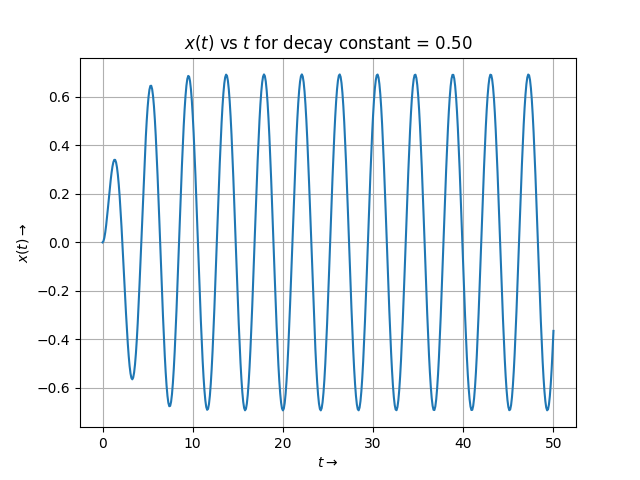
\includegraphics[scale = 0.8]{Figure_1.png}
    \label{fig:sample}
\end{figure}
\begin{center}
    The decay in the response dies out after sometime and the response becomes
purely sinusoidal
\end{center}
\vspace*{-0.5cm}
\begin{figure}[H]
    \centering
    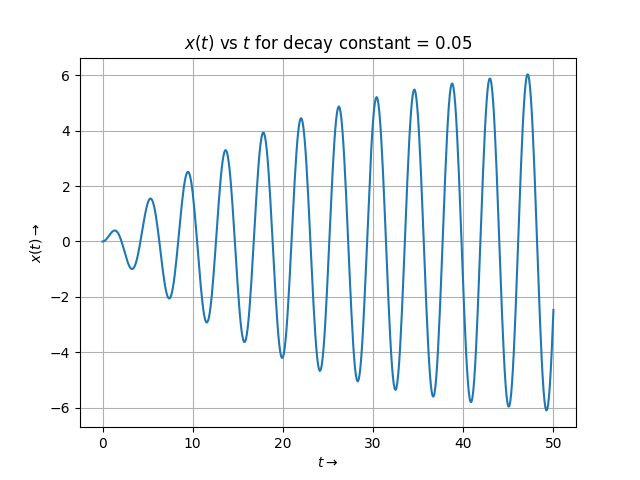
\includegraphics[scale = 0.8]{Figure_2.png}
    \label{fig:sample}
\end{figure}
\begin{center}
    The decay dies in this graph as well but takes more time to vanish since the
decay constant is low compared to the previous plot
\end{center}
\subsection{Response of the spring-mass system for different frequencies}
\vspace*{-0.5cm}
\begin{figure}[H]
    \centering
    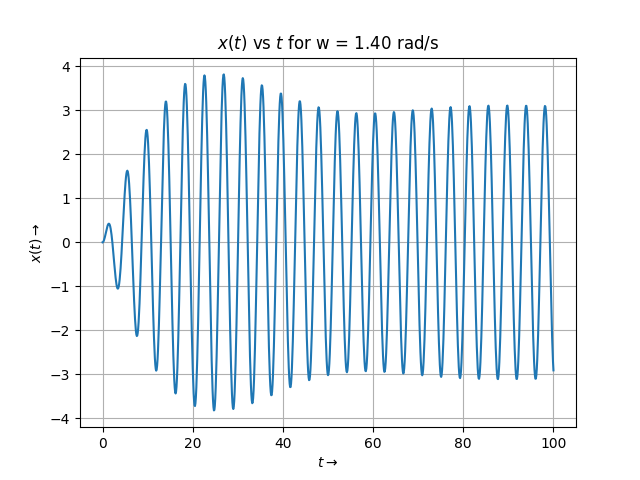
\includegraphics[scale = 0.9]{Figure_3.png}
    \label{fig:sample}
\end{figure}
\vspace*{-0.5cm}
\begin{figure}[H]
    \centering
    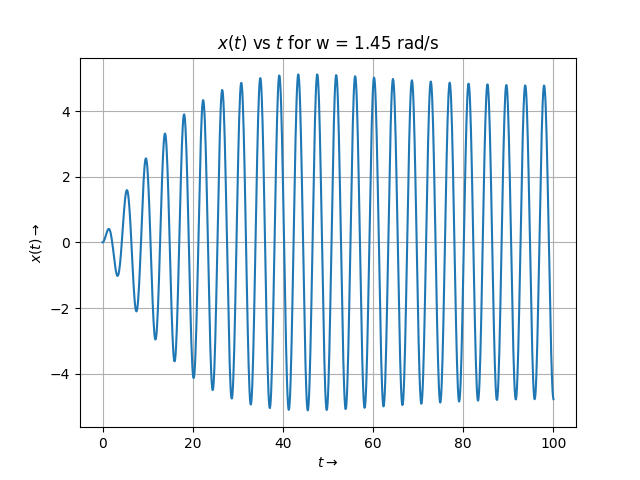
\includegraphics[scale = 0.9]{Figure_4.png}
    \label{fig:sample}
\end{figure}
\vspace*{-0.5cm}
\begin{figure}[H]
    \centering
    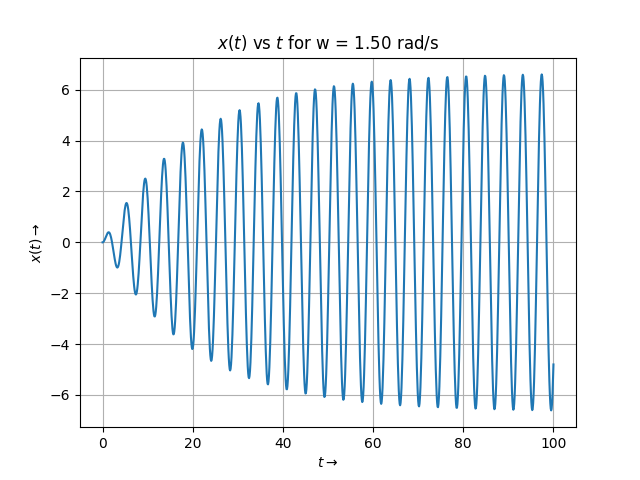
\includegraphics[scale = 0.9]{Figure_5.png}
    \label{fig:sample}
\end{figure}
\vspace*{-0.5cm}
\begin{figure}[H]
    \centering
    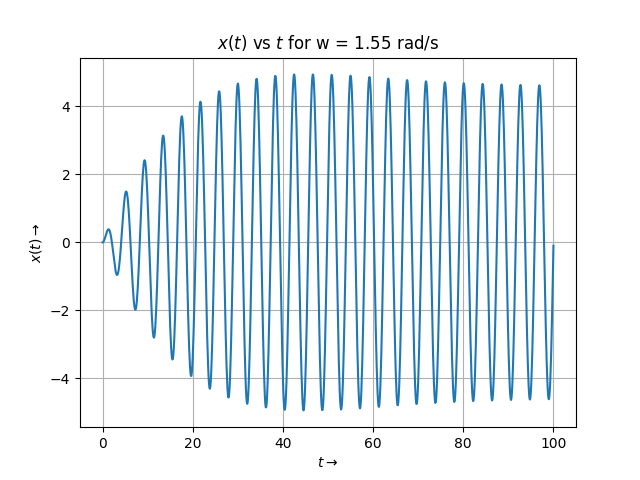
\includegraphics[scale = 0.9]{Figure_6.png}
    \label{fig:sample}
\end{figure}
\vspace*{-0.5cm}
\begin{figure}[H]
    \centering
    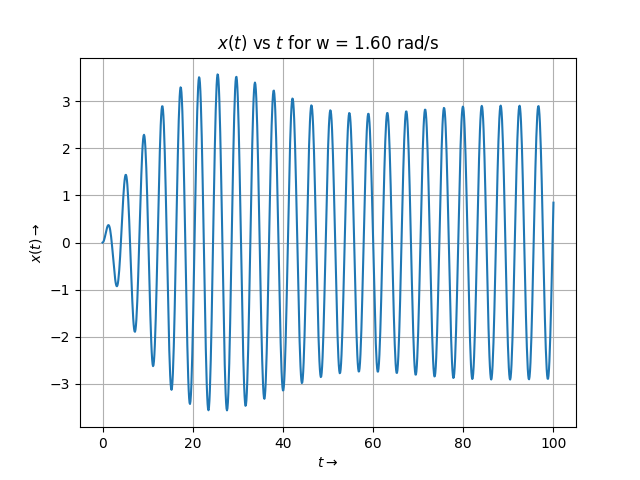
\includegraphics[scale = 0.9]{Figure_7.png}
    \label{fig:sample}
\end{figure}
Clearly the response is having maximum amplitude for $\omega = 1.5$ rad/s. It is obvious since the resonant frequency of the spring-mass system is $\sqrt{2.25} = 1.5$ rad/s 
and that is equal to the driving frequency as well. Hence, the response is maximum at $\omega = 1.5$ rad/s and starts to attenuate for frequencies around it.
\subsection{Coupled Spring Problem}
The coupled differential equations corresponding to the responses of two springs are given as follows:
\begin{equation*}
    \ddot xx+x-y=0 
\end{equation*}
\begin{equation*}
    \ddot y+2(y-x)=0
\end{equation*}
Solving for $X(s)$ and $Y(s)$ with inital conditions as $x(0)=1,\ \dot x(0)=\dot y(0)=y(0)=0$, we have:
\begin{equation*}
    X(s) = \frac{s^{2}+2}{s^{3}+3s}
\end{equation*}
\begin{equation*}
    Y(s) = \frac{2}{s^{3}+3s}
\end{equation*}
These laplace transform expressions are again converted back to time domain and the time responses are obtained in the plot given below:
\begin{figure}[H]
    \centering
    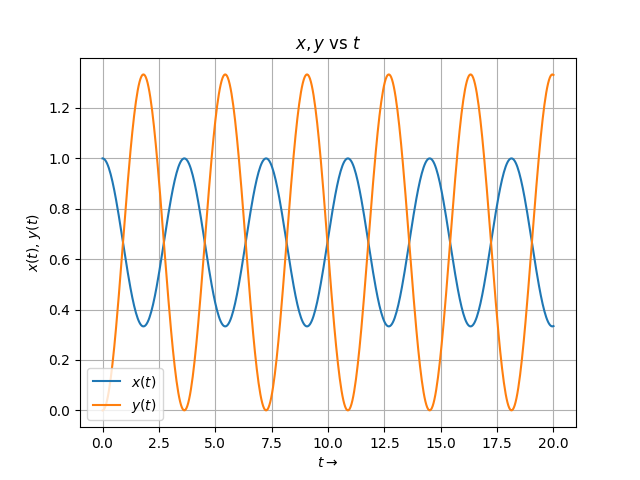
\includegraphics[scale = 0.8]{Figure_8.png}
    \label{fig:sample}
\end{figure}
\begin{center}
    Both the springs have sinusoical responses with the response of $y$ being more in amplitude than that of $x$. The reason is simple: $y(t) = 2(u(t)-x(t))$
\end{center}
\subsection{RLC Filter}
This is an electrical engineering example. The objective is to analyze the frequency domain gain and phase of the transfer function of the system shown below:
\begin{figure}[H]
    \centering
    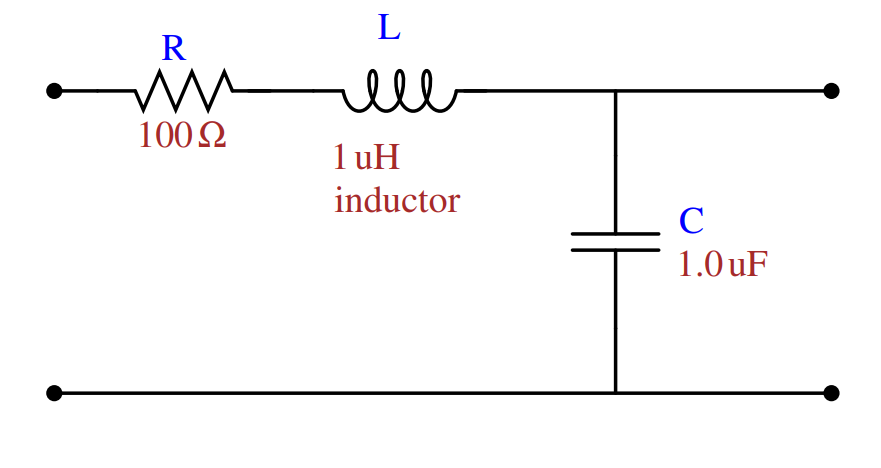
\includegraphics[scale = 0.8]{Figure_rlc.png}
    \label{fig:sample}
\end{figure}
The transfer function of this system is:
\begin{equation*}
    H(s) = \frac{1}{s^{2}LC+sRC+1}
\end{equation*}
where $R = 100 \Omega$, $L = 1\mu H$ and $C = 1\mu F$. The magnitude and phase reponse plots are shown below:
\begin{figure}[H]
    \centering
    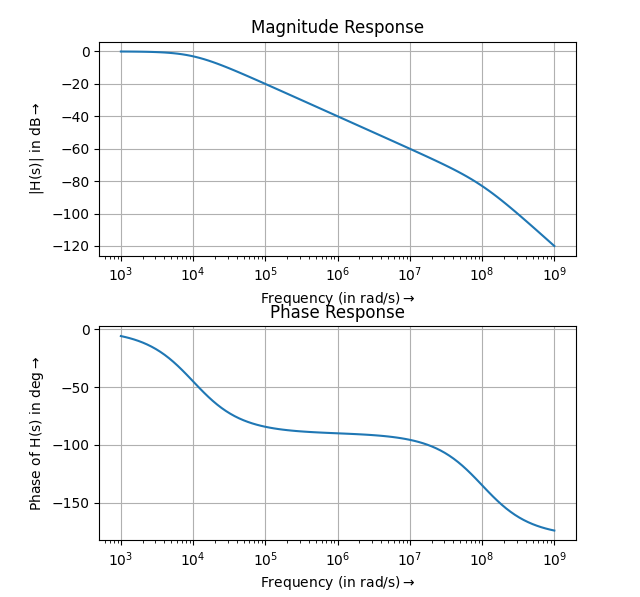
\includegraphics[scale = 1]{Figure_9.png}
    \label{fig:sample}
\end{figure}
Now an input voltage is applied to this system. The input voltage expression is given as:
\begin{equation*}
    v_{i}(t) = \cos(10^{3}t) - \cos(10^{6}t)
\end{equation*}
Converting this to the laplace form, multiplying it with the transfer function and then inverting the result back to the time domain, we have the following graphs:
\begin{figure}[H]
    \centering
    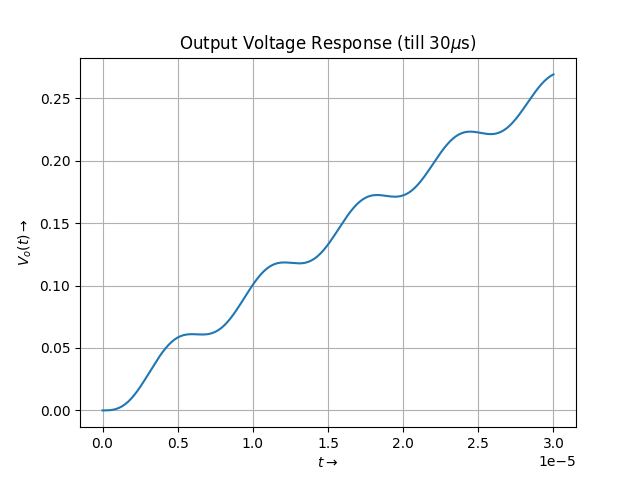
\includegraphics[scale = 0.8]{Figure_10.png}
    \label{fig:sample}
\end{figure}
\begin{center}
    The response is steadily increasing with slight sinusoidal variations
\end{center}
\vspace*{-0.5cm}
\begin{figure}[H]
    \centering
    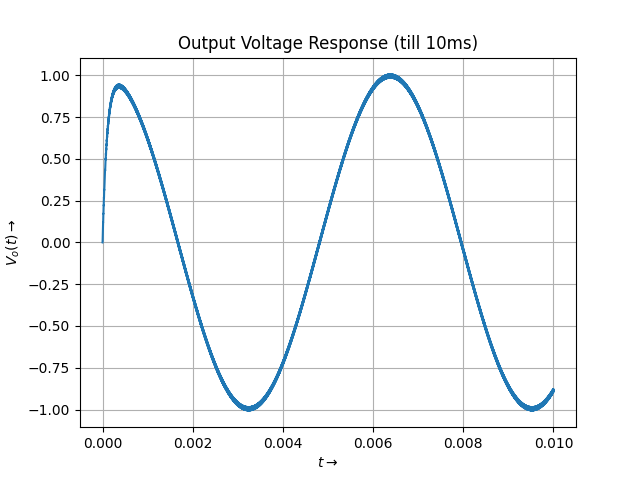
\includegraphics[scale = 0.8]{Figure_11.png}
    \label{fig:sample}
\end{figure}
\begin{center}
    The response looks almost sinusoidal with frequency of $1000$ rad/s
\end{center}
\vspace*{-0.5cm}
\begin{figure}[H]
    \centering
    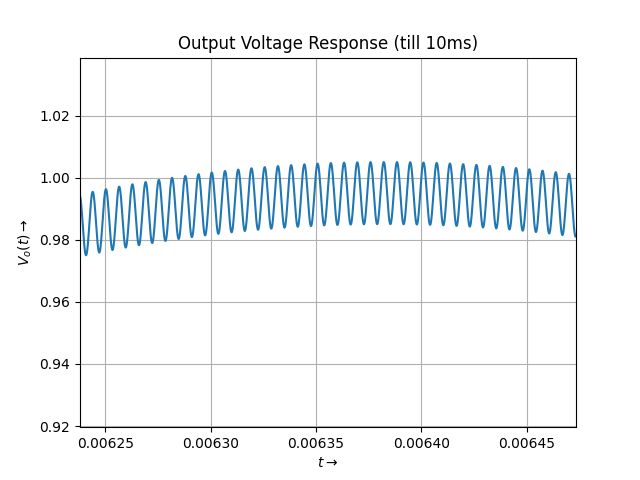
\includegraphics[scale = 0.8]{Figure_11_2.png}
    \label{fig:sample}
\end{figure}
\begin{center}
    On zooming, we can see that there are small sinusoidal variations on the top of the sinusoidal graph obtained in the previous figure.
\end{center}
\section{Conclusions}
\begin{enumerate}
    \item The time responses of the spring mass system in Q1 and Q2 reach steady state and have a sinusoidal variation. The exponential components decay after some time and the time taken to reach steady state is less in case of $a=0.5$ as expected.
    \item In Q3, the response has maximum amplitude at $\omega = 1.5$ rad/s since that is equal to the resonant frequency of the spring-mass system. Frequencies other than $1.5$ rad/s have lower amplitudes.
    \item In Q4, the response of spring Y is having more amplitude than that of spring X since $y(t)=2(u(t)-x(t))$. Both the responses are sinusoidal with $\omega = \sqrt{3} = 1.732$ rad/s.
    \item In Q5, from the magnitude and phase responses, it is evident that the filter is a second order low-pass filter with its pole frequencies as $p_{1}=10^{4}$ rad/s and $p_{2}=10^{8}$ rad/s. Hence, it is a real pole system and hence, the magnitude response is a strictly decreasing function.
    \item In Q6, the output voltage clearly is dominated by the component of $\omega = 10^{3}$ rad/s and this is obvious since $10^{3}$ is less than the first pole frequency, $10^{4}$. However, the component of $\omega = 10^{6}$ rad/s is very low and it just acts as noise to the output.
\end{enumerate}
\end{document}